\documentclass[journal]{IEEEtran}
\usepackage{amsmath,amssymb,amsfonts}
\usepackage{algorithmic}
\usepackage{algorithm}
\usepackage{array}
\usepackage[caption=false,font=normalsize,labelfont=sf,textfont=sf]{subfig}
\usepackage{textcomp}
\usepackage{stfloats}
\usepackage{url}
\usepackage{verbatim}
\usepackage{graphicx}
\usepackage{gensymb}
%\usepackage{times} used initially but stopped when using latest TMECH journal formatting guidelines.
%\usepackage{comment} used initially but stopped when using latest TMECH journal formatting guidelines.
%\usepackage{urwchancal} trying to fix \mathpzc undefined control sequence issue.
\usepackage{cite}
\hyphenation{op-tical net-works semi-conduc-tor IEEE-Xplore}
% updated with editorial comments 8/9/2021

\begin{document}

\title{A Compliant Rolling Ellipsoidal Thumb Joint for the TU Hand}

\author{Spenser Pulleyking,~\IEEEmembership{Student Member,~IEEE}, Joshua Schultz,~\IEEEmembership{Senior Member,~IEEE}
        % <-this % stops a space
\thanks{All authors are with the Department of Mechanical Engineering, The University of Tulsa, Tulsa, OK 74104, USA (e-mail: spenser-pulleyking@utulsa.edu; joshua-schultz@utulsa.edu). Research supported by NSF NRI 1427250.}% <-this % stops a space
\thanks{Manuscript submitted March 1, 2023.}}

% The paper headers

%\markboth{Journal of \LaTeX\ Class Files,~Vol.~14, No.~8, August~2021}%
%{Shell \MakeLowercase{\textit{et al.}}: A Sample Article Using IEEEtran.cls for IEEE Journals}

\markboth{IEEE/ASME Transactions on Mechatronics}%
{Shell \MakeLowercase{\textit{et al.}}: A Compliant Rolling Ellipsoidal Thumb Joint for the TU Hand}

%\IEEEpubid{0000--0000/00\$00.00~\copyright~2023 IEEE}
% Remember, if you use this you must call \IEEEpubidadjcol in the second
% column for its text to clear the IEEEpubid mark.

\maketitle

\begin{abstract}
This work presents a compliant rolling ellipsoidal carpometacarpal (CMC) joint for the thumb of a robotic hand. This work is the first to introduce the Bi-Ellipsoidal joint, a flexure hinge-based biomimetic thumb CMC joint. A model of this design is implemented in simulation and in experiment, and compares the Manipulability Metrics, a quality metric for the end-effectors within robotic manipulators, across similar workspaces. Compliant mechanisms known as flexure hinges maintain the 3D rolling of the ellipsoids rather than sliding or slipping. By comparing the results for the Bi-Ellipsoidal joint with a gimbal joint, the relative size and location of the region of highest manipulability was found to be similar between CMC joint models, although the shape of this region varied somewhat from one to the other. The experimental comparison used tendon-displacement data generated from bio-inspired hardware prototypes of both the Bi-Ellipsoidal CMC joint and gimbal CMC joint models for two similar robotic thumbs, while the analytical version used iterative forward kinematics to derive and compare the Manipulability Metric distributions. 
\end{abstract}

\begin{IEEEkeywords}
Robotics, Biomimetic and bio-inspired robotics, Grasping and manipulation.
\end{IEEEkeywords}

\section{Introduction}
\IEEEPARstart{T}{he} usefulness of biological hands emerges subtly from underlying relationships in a compliant network of rigid and soft bodies, tendons, and ligaments. Thumb use exploits this while controlling our own hand, but research is still exploring how simplified inputs can model complex grasping tasks \cite{moravec}. Our anatomy utilizes kinematic coupling via underactuation: a state of a system where fewer inputs exist than outputs, in a compliant network comprised of tendons, bearings, and flexure hinges. Underactuation makes devices conform to the shape of the object being grasped; this may contribute to the inverse correlation between any given tool's ubiquity and prevalence in human tasks, and the number of its degrees of freedom \cite{Martell, Fuzzy}. %This improves our ability to grasp objects, as we can control our thumb motion lateral to the palm (flexion/extension) as well as transverse to it (adduction/abduction), while the thumb's pulp maintains its inward orientation through pronation and/or supination \cite{anatomy-textbook}.

Starting from the palm, the anatomical joints of the thumb are commonly referred to as the carpometacarpal (CMC), the metacarpophalangeal (MCP), and the interphalangeal (IP) joints. Treating the IP joint as mobile, the MCP joint as fixed, and the CMC joint as rolling without gliding or slipping, the device is implemented in The University of Tulsa Anthropomorphic Robotic Hand, or the TU Hand \cite{Pulleyking}, \cite{Pulleyking-Schultz}, \cite{Das-TUHand}. Biological joints' connective tissue allows limited shearing-motions between contact surfaces of bones: there is a strong preference for minimizing slipping during rolling, which may also allow for more precise kinematic motions \cite{anatomy-textbook}. Due to the CMC joint's high level of interpersonal variability, there is also significant disagreement on a discrete assignment of the location and orientation of the axes of revolution or translation \cite{noparams}. This region, sometimes known as the Trapezio-Metacarpal complex, consists of interactions between eight bones and twelve ligaments. This complexity affects reducing the biological mechanism into a system of traditional joints. Alternatively, this complex cannot be defined as a Reuleaux kinematic pair, further precluding biomimetic design approaches \cite{reuleaux}. 

 Using a gimbal (perpendicular joint with intersecting axes) in robotic hands appears to be one of the most common CMC joint 2-DoF configuration. A list of anthropomorphic robotic hands with gimbal thumb CMC joints includes the {\it AllegroHand}, {\it ShadowHand}, and {\it iCub} biomimetic robotic hands \cite{ShadowHand}, \cite{iCub}, \cite{KITECH-Hand}. The notion of a gimbal is based on a pair of orthogonal degrees of freedom, and is often at the core of state of the art thumb CMC joint design. While these thumbs may not be considered to be biologically inspired, their design may benefit from the symmetry in the sensors of their similar opposing digits, which precludes the need to design an independent thumb model \cite{DLRhand}, \cite{schunkhand}. In addition to recent commercially-available myoelectric prostheses, arthrodesis (joint fixation at a specific pose) is also being used to take advantage of simplified design to preserve functionality \cite{bebionic}. As in prior work, the MCP joint is treated as fixed to reduce complexity \cite{Pulleyking}. No research to the author's knowledge has yet explored the influence of arthrodesis on manipulability within an underactuated device. Underactuated robotic hands systems are simpler to control than fully-actuated equivalent systems \cite{AdaptUnderact}. 

 %This phenomenon should not be considered separately from the underactuation we observe biologically, in that the underactuation of the device simplifies not only the assemblies required to guarantee the desired kinetic motion, but also simplifies the problem from a control perspective: instead of seeking path-planning solutions in a full-dimensional space of all possible equilibrium points accessible under smooth feedback stabilization as a fully actuated device must consider, underactuated devices' feedback schemes achieve stabilization which is restricted to a manifold sub-set of the overall space of equilibrium point solutions \cite{Oriolo-Nakamura}. 

%The Bi-Ellipsoidal joint may provide some safety advantages to the design of a bioinspired hand, but these cannot be useful

Hybrid soft-rigid robotic grippers conform to objects during manipulation, without complex planning of each phalanx's position and orientation \cite{softrigid}. To measure the ability of a digit, such as grasping or in-hand object manipulation, the Manipulability Metric (MM) quantifies the ability of an end effector to be moved smoothly in any direction in the workspace \cite{Yoshikawa}. Many uses of the Manipulability Metric exist: one extension is the dynamic Manipulability Metric, which can be used to evaluate dynamic grasping \cite{yokokohjiDME}. Our system of the tendon-driven thumb is designed to reduce complexity without substantially reducing function, taking inspiration from the biological TM complex. Prior to this paper, this work was partially published only to develop the Simplified Manipulability Metric (SMM), a quick approximation of the MM. \cite{Pulleyking-Schultz}. 

The organization of the paper is as follows. In Section \ref{flexhinge}, a compliant mechanism is presented to constrain the internal components of two rolling ellipsoids that constitute a 2-DOF thumb CMC joint. In Section \ref{manoftde}, the application of this metric to a tendon-driven system is established, and two Jacobians are computed to inform the Manipulability Metrics of our tendon-driven and joint-angle systems. In Section \ref{mechd}, the prototype hardware is described as it pertains to this experiment. In Section \ref{kinmodel}, kinematic models for both our rolling ellipsoidal CMC joint and a gimbal CMC joint are presented. In Section \ref{dhsection}, the Denavit-Hartenburg parameters for the models are developed and discussed. In Section \ref{datasection}, the data collection and procedure are described for gathering the end-effector and tendon displacement data throughout the experimental workspace. In Section \ref{results}, the Manipulability Metrics are calculated, and in Section \ref{discussion} the results of the analytical and simulated experiments are discussed. Section \ref{conclusion} presents a summary of this work and paths toward future work.

%OLD Outline: Sections: NEEDS UPDATE

%1) Manipulability of Tendon-Driven End-Effectors
% A) Thumb Arthrodesis
% B) The gimbal CMC joint Model
%2) Experimental and Simulated Bi-Ellipsoidal Rolling Carpo-Metacarpal Joint
% A) Ellipsoidal Rolling Joint Kinematic Model
% B) Comparison via Denavit-Hartenberg Parameters
%3) Prototype Experiment
% A) Materials and Structural Design
% B) Data Collection Procedure
%4) Two Jacobian Formulations to Calculate the Manipulability Metric
%5) Results
% A) Joint Space to Task Space Manipulability Metric
% B) Tendon Extension to Task Space Manipulability Metric



\section{Compliant Flexure Hinges to Constrain Rolling Ellipsoids}

\label{flexhinge}

When two ellipsoids are in contact, to constrain constant lengths between the opposing foçi is challenging, as sliding may occur at the contact point. We present a pair of compliant mechanisms with flexure hinges to join the foçi such that both abduction-adduction and flexion-extension motion can occur. Flexure Hinges are components that constrain angular motion during elastic material deformation; as such they produce many advantages common to compliant mechanisms, such low friction and high sensitivity \cite{fhdef}. This means that the rolling motion for abduction-adduction can occur within the ellipsoids' carriage, but the foçi are held a fixed distance apart at all poses as described by Blake et. al, ``each focus of the one remains at a constant distance, viz. the transverse axis of one of the ellipses, from a focus of the other." \cite{Blake}. The flexure hinges also provide a restoring force that will center the joint when unloaded.

\begin{figure}
	\centering
	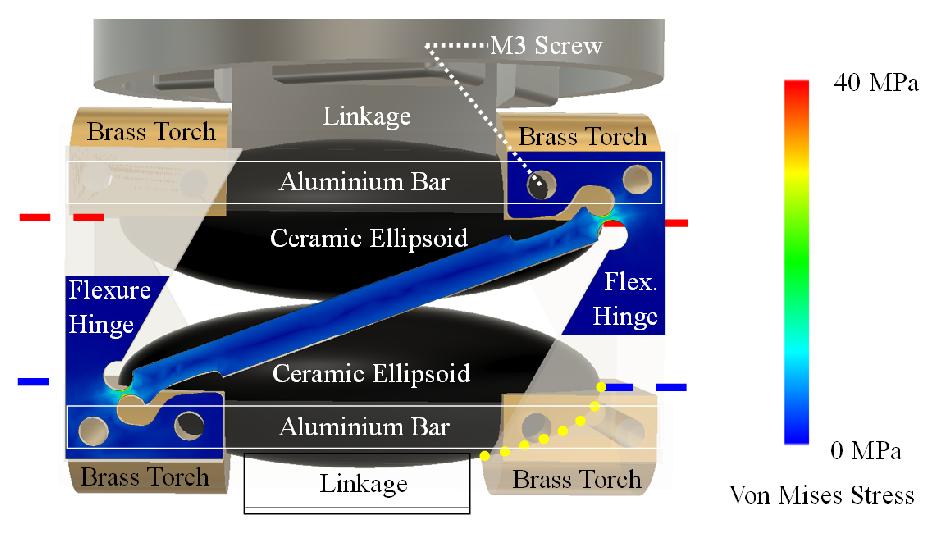
\includegraphics[width = 1\columnwidth]{figures/vonmises2.eps}
	\caption{A close-up image of a CAD model for the Bi-Ellipsoidal joint which highlights the Von-Mises stresses in one of the flexure hinges.}\label{torches}
	%%
 \label{vonmises}
\end{figure}

Polypropylene was selected for the material. A finite element analysis was performed on the final flexure hinge design, which confirmed that the flexure hinge was well within the bounds of elastic deformation for the given material and geometry, as shown in Figure \ref{vonmises}. The C-type hinges are shown to have stress concentrations and may host some deformation, but the geometry tolerates it while restricting the overall motion as desired. 

 In tandem with the flexure hinges, four brass ``torches" were created to house the ends of the ellipsoids: together, this sub-assembly forms a ``carriage" for the motion of the ellipsoids. As the torches are linked to the flexure hinges with screws, the prolate ends of the ellipsoids within the torches are constrained by similar kinematics, so that the ellipsoids cannot exit the torches, as shown in Figure \ref{torches}. The torches are linked to the flexure hinges and are linked by thin aluminium crossbars: together, the constraints imposed fully define the position of both ellipsoids. The brass torches' inner profile is highlighted on one of the four torches with a dotted yellow line in Figure \ref{vonmises}. The lower base ellipsoid is embedded below the surface of the palm, and the upper ellipsoid is embedded in the metacarpal bone of the thumb, so the contact surface will consist of only a sub-region of one semi-ellipsoid of each, as shown in Figures \ref{torches} and \ref{thumbphoto}. 


\section{Manipulability of Tendon-Driven End-Effectors}

\label{manoftde}
\begin{equation} 
\hspace{40pt} MM = \sqrt{\mathrm{det}(J(\theta )J(\theta )^{T})} 
 \label{eq1}
\end{equation}

%%{10pt}

A set of four Manipulability Metric distributions are calculated: 

%%{10pt}

\begin{itemize}
 \item Tendon manipulability (ellipsoidal)
 \item Tendon manipulability (gimbal)
 \item Standard (joint-task space) manipulability (ellipsoidal)
 \item Standard (joint-task space) manipulability (gimbal)
\end{itemize}

%%{10pt}

%This paper's approach to finding Manipulability is similar to the recent analysis of the KITECH Hand, which is a research application of the earlier Allegro Hand, a fully-actuated robotic research prototype: while that work focused uniquely on calculating `Thumb Opposability' and studying dexterous manipulation of all five fingers together, this paper focuses on the effect joint design has on the manipulability of the thumb \cite{KITECH-Hand}. %Furthermore, a reduced data set is used to speed calculation: 120 000 points are sampled throughout the workspace, which is less than one-quarter of the previous method.

%\section{Manipulability}

We develop standard forward kinematics to predict the joint angles' correspondence with the end-effector's position, while also measuring tendon displacement. Each path will produce a distinct version of the Jacobian to consider when calculating a Manipulability Metric for our thumb: the joint space to task space matrix, and the tendon excursion to task space matrix. This is due to the use of a tendon-drive mechanism with inextensible tendons. The Jacobian derived from joint space and the Jacobian derived from tendon excursion will each be generated and discussed, in the context of both experimental verification with a physical prototype, and with a computer simulation using a symbolically-generated data-set based on the forward kinematics of both CMC joint prototypes. %In either case, the essential role of the Manipulability Metric is to compare Eigenvalues' ratios to each other, which is why the Manipulability Metric is utilized.
%Because the Manipulability Metric also represents an ellipsoid-volume for a given pose of the thumb, the summation of all points can represent the total volume of all manipulability ellipsoids at all points. 

The fact that the MCP is a fixed joint, in both the model of the joint angles and the physical prototype, is as inspired by surgical arthrodesis \cite{Pulleyking}, \cite{Pulleyking-Schultz}. While this reduces the manipulability of the individual fingertip, this drastically reduces the complexity of the device. As the MCP joint is fixed in both cases, the Manipulability Metric will be compared between the rolling CMC joint introduced here and the gimbal CMC joint, and the benefits of the two designs will be considered.

\begin{table}
 \centering
 \caption{Angle Measurements are shown in Degrees.}
 \begin{tabular}{c|c|c}
	Structure & Variable & Length (mm) \\
	\hline
	Metacarpal & $\ell_{mcp}$ & 74.63 \\
	Proximal Phalanx & $\ell_{pp}$ & 27.88 \\
	Distal Phalanx & $\ell_{dp}$ & 34.26 \\
	\hline
	\hline
	\end{tabular}
 \begin{tabular}{c|c|c}
 Degree of Freedom & Variable & Range of Motion (deg)\\
	\hline
	CMC Joint Flexion/Extension & $\mu$ & $0\degree\leftrightarrow70\degree$\\
	CMC Joint Abduction/Adduction & $\sigma$ & $-20\degree\leftrightarrow20\degree$\\
	IP Joint Flexion/Extension & $\omega$ & $-15\degree\leftrightarrow80\degree$\\
	\hline
	\hline
	\end{tabular}
 \label{jointdegrees}
\end{table}

The Jacobian matrix functions in robotics as a mapping between the joint-angle velocities and the velocity of the end effector in the workspace, but in principle, it can be applied to quantities other than the joint space variables, such as tendon excursions. Our prototypes will go on to demonstrate that a Jacobian and corresponding Manipulability Metric derived from tendon-displacement inputs in place of joint angle information will produce similarly useful results. The tendon-based Jacobian used to calculate the Manipulability Metric for our two physical prototypes, $J_{A}$, is shown in Equation \ref{eq2}, and the traditional joint-based Jacobian used to calculate the Manipulability Metric for our two analytical simulations, $J_{T}$, is shown in Equation \ref{eq2T}: as it uses joint angles as input, the variables are the same as those used in Table \ref{jointdegrees} to define a kinematic model.

%Jt = 3x4 matrix (eq 3)
\begin{equation} 
%\hspace{40pt} 
J_{A} = \begin{bmatrix}

\frac{\delta x}{\delta d_{1}} & \frac{\delta x}{\delta d_{2}} & \frac{\delta x}{\delta d_{3}} & \frac{\delta x}{\delta d_{4}} \\ 

\frac{\delta y}{\delta d_{1}} & \frac{\delta y}{\delta d_{2}} & \frac{\delta y}{\delta d_{3}} & \frac{\delta y}{\delta d_{4}} \\ 

\frac{\delta z}{\delta d_{1}} & \frac{\delta z}{\delta d_{2}} & \frac{\delta z}{\delta d_{3}} & \frac{\delta z}{\delta d_{4}}
 
\end{bmatrix} 
%\hspace{40pt} 
\label{eq2}
\end{equation}

\begin{equation} 
%\hspace{40pt} 
J_{T} = \begin{bmatrix}

%%{1pt}\frac{\delta x}{\delta \mu} & \frac{\delta x}{\delta \sigma} & \frac{\delta x}{\delta \omega} \\ 
%%{1pt}
\frac{\delta y}{\delta \mu} & \frac{\delta y}{\delta \sigma} & \frac{\delta y}{\delta \omega} \\ 
\frac{\delta z}{\delta \mu} & \frac{\delta z}{\delta \sigma} & \frac{\delta z}{\delta \omega} 
 
\end{bmatrix} 
%\hspace{40pt} 
\label{eq2T}
\end{equation}

For the tendon-based Jacobian matrix in Equation \ref{eq2}, there are two independent columns: one for coupled flexion/extension of the CMC joint and IP joint, and one for the abduction/adduction of the CMC joint. As we introduce this ``tendon-Jacobian" $J_{T}$, it should be contrasted with the standard Jacobian. The tendon-Jacobian was evaluated by sampling the experimental data, whereas the standard Jacobian is generated by sampling the kinematic model. %The flexion and extension tendons mirror each other's travel distance, and the abduction and adduction tendons do the same. 

From a tendon networking perspective, by the application of Caratheodory's theorem, four actuators are sufficient to fully actuate three joints, given certain tendon configurations, and assuming that each tendon needs one actuator to pull it separately \cite{MLS}. Alternatively, each of the four tendons of our three-joint prototypes is designed to share with another tendon; thus, for four tendons, only two sources are required \cite{malhotra}. By configuring two pairs of opposing tendons, one pair being flexion/extension and the other adduction/abduction, one point of actuation can simultaneously pull two tendons in opposite directions. The fixture of the MCP joint dictates the remaining degrees of freedom, as seen in Table \ref{jointdegrees}. 

%\subsection{Thumb Arthrodesis}

%Due to their constant usage and our vulnerable biology, the health of the thumb joints is a critical component of any individual's quality of life. When arthritis, or other joint damage and irritation, occur in these joints, it is still sometimes the best surgical practice to fuse one or more joints as fixed together, or into a mechanical coupling with reduced degrees of freedom, termed Arthrodesis \cite{Pulleyking}.

%While there is some expectation for reduced functionality and dexterity while grasping and manipulating objects in the hands when an Arthrodesis has been performed, some joints generally respond better to arthrodesis than others. Optimal angles for these mechanical interventions have heuristically emerged through surgical practice: specifically, arthrodesis of the thumb's metacarpal (MCP) joint produced acceptable patient outcomes, both when the joint was statically fused, and when the range of motion was significantly reduced, for given angular parameters. As shown in Figure \ref{thumbphoto}, our prototypes' MCP joints are fixed, which allows the fusion of the surrounding linkages into one. %While previous research hoped to extract from this data how the parameters of the {\it Steiger Arthrodesis}, a total fusion of the MCP joint, could be implemented into a biomimetic robotic thumb to offer a drastic mechanical and structural simplification without removing functionality. 
%Unlike the biological hand, which requires surgical intervention to avoid damaging its complexity during repairs, robotic hand assemblies should be designed to be accessible, and thus mechanical simplicity is desirable. This is because the fusion of two bodies--which previously were actuated and coupled by a complex interaction of  twelve different tendons, ligaments, and connective tissue structures--removes many components, assembly steps and failure points to any biomimetic thumb prototype [2].
%From Biorob 2016: REQUEST PERMISSION TO RE-USE (caption is copied directly, is this ok?)
%Figure: Photo of the thumb
%Although our previous research shows a reduction in workspace volume occurs after performing thumb metacarpophalangeal joint arthrodesis, there was a beneficial simplification of the underlying kinematics, which allows for a more robust mechanical device \cite{Pulleyking}, \cite{Pulleyking-Schultz}. 

%Towards this goal, our thumb is designed to dislocate under a greater load than it is rated for; what this means in terms of safety is that some guarantees can be expected about the total possible output of the device. 
%Figure: Photo of the thumb

\begin{figure}
	\centering
	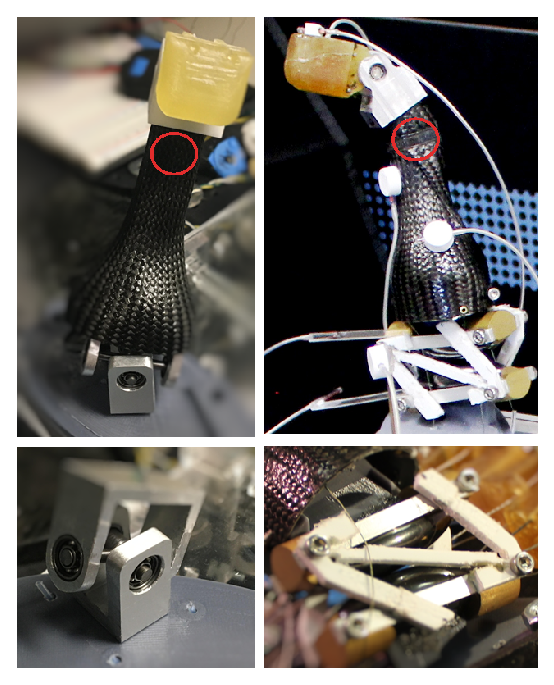
\includegraphics[width = 1\columnwidth]{figures/four_panel-two_models.eps}
	\caption{Left: The reference thumb is designed with a traditional gimbal-like carpometacarpal joint, made from aluminium and steel. Right: the Bi-Ellipsoidal carpometacarpal joint introduced in this paper. As the phalanges around the MCP joint are fused into a single linkage as inspired by arthrodesis, the MCP joint's location is highlighted in both with a red circle.}
 \label{thumbphoto}
	%%
\end{figure}

%When searching for anthropomorphic designs, PRIOR WORK: Where does this work sit with regard to the prior work? Ours? DLR Hand papers (remember: Hyperboloid-type joint) Valero-quevas, santos, steiger arthrodesis, other anthro/biomimetic thumbs out there since I last checked? 

%\subsection{Thumb CMC joint prototype simplifications and the TU Hand}

\section{Mechanical Design}

\label{mechd}
 The Bi-Ellipsoidal joint hardware developed for the experimental section can be seen installed on the {\it TU Hand}, a research platform for similar experimental hardware \cite{Rake-Tendons}, \cite{rake2}. Many variants of similar rolling congruent parametric surfaces can be found in various industrial applications and designs, such as elliptical gear/diaphram meshes, as the mathematical relationship between such general surfaces is well established \cite{Blake}. An in situ view of this assembly and of a gimbal CMC joint can be seen in Figure \ref{thumbphoto}. The gimbal CMC is constructed from u-channel brackets with press fit bearings and two orthogonal pin joints that support the two perpendicular shafts, which are fixed together at their intersection. 

For the ellipsoids in our Bi-Ellipsoidal prototype we use pseudo-ellipsoidal ceramic magnets that are available at low cost. These are known as the ``Rattlesnake Eggs" toy, and embody ellipsoidal surface contact patches. As outlined in Section \ref{flexhinge}, the ellipsoids' carriage is manufactured from aluminium, brass, and polypropylene. To best understand how such a network of couplings can be realized in hardware, first consider the 2D case seen in Figure \ref{2dc}. The cross-linkages, represented by segments $BC$ and $AD$, are chosen to enforce a constant distance between the crossed foçi of the ellipses. Now considering the 3D version: unlike the 2D version, we can not put a pivot through each focus, as the ellipsoid needs to roll about its major axis in the flexion-extension direction. We need some other way to constrain the foçi so they remain a constant distance from one another as they move, without hindering the rolling in the flexion-extension direction. The key aspect is that the ellipsoids are able to abduct and adduct as shown in Figure \ref{spacesymbol}b, as well as roll about their major axes, and thus constrain the motion imparted by the four tendons traversing the joint, such that the device has a biomimetic range of motion. As seen in Figure \ref{thumbphoto}, a rigid link termed the MCP Fusion is comprised of the metacarpal fused to the proximal phalanx at the angles of the Steiger Arthrodesis: $15^{\circ}$ flexion, $10^{\circ}$ pronation (adduction) \cite{Pulleyking}. Thin-walled carbon fiber layup was precisely molded to the desired angle of arthrodesis at the MCP joint using an internal 3D printed scaffold upon which to mold the fiber's geometry as the resin cures. To do this, a woven carbon fiber sleeve that narrows as it is stretched was held with a weight to conform to the 3D printed geometry. %This process was identical between both the rolling ellipsoid and gimbal thumb prototypes. 


\begin{figure}
	\centering
	%%{7pt}
	\includegraphics[width = 1\columnwidth]{figures/ellipsediagramv3-2.eps}
	\caption{(a) A 1-DoF Hinge joint and its resulting curved workspace. (b) A 1-DoF Bi-Ellipse Joint and its resulting workspace.}
 \label{2dc}
	%%
\end{figure}

The brass and Aluminium components, respectively labeled the `torch' and crossbar, are rigidly coupled together with M3 screws to cage the ellipsoids as they roll and contact the inner torch-shape surfaces, without obstructing their linkage which extends outside the cage: thus, the boundaries of this rigid body become the mechanical stops of the joint, as shown in Figure \ref{vonmises}. The top and bottom ellipsoid cages are also coupled by two flexure hinges, whose white polypropylene surfaces can be seen around the CMC joint in Figure \ref{thumbphoto}. These two C-type flexure hinges are to enforce necessary kinetostatic linkage, acting together as a composite compliant mechanism \cite{fhdef}. They were milled out from a \(\frac{1}{8}\)" sheet of standard grade polypropylene on a {\it HAAS Mini Mill}. 

%For the comparative model joint prototype, a traditional gimbal is developed and assembled to represent the thumb CMC joint: a cross-shaft is pressed through a main shaft, and both shafts are supported by an upper and lower aluminum u-channel bracket machined for the prototype. 

%%When the ellipsoids were first realized in a prototype via the "Rattlesnake Eggs", the magnetic interaction between them cannot hold them together when the thumb is under load. If there was no magnetic field, just the ellipsoidal geometry, ligaments would be necessary to mechanically couple the surfaces' motion together, into rolling without slipping. The crossbars and torches, realized in Aluminium and Brass, prevent slipping in the lateral direction. %However, twin prolate ellipsoids have been shown to be coupled by the aforementioned ellipsoidal coupling at the foçi, which show an input-reversible interaction between the input to the joint and the position of the contact point between the ellipsoids. %What happens when force transmission between the ellipsoids increases? If they are deformable under such a load, how does the increased contact surface area from deformation affect the potential slip between them? For now, we only consider rigid surfaces, but it is possible to better understand the geometric relationship using point-clouds generated from forward kinematics.

%, including the {\it AllegroHand}, {\it ShadowHand}, and {\it iCub} biomimetic robotic hands \cite{ShadowHand}, \cite{iCub}, \cite{KITECH-Hand}.

%\begin{comment}
%While the Manipulability Metric is a powerful tool to predict the dexterity of a manipulator at a given point in its workspace, the application of this metric to in-hardware grasping experiments has so far been limited to fully-actuated hands, which are not as biomimetic as underactuated manipulators such as the {\it TU Hand} \cite{Chen}. There is a clear need for this cross-application of the predictive metric, as underactuated biomimetic hands (or fully-actuated robotic hands constrained by parametric equations in software) are an active area of research in biologically inspired robotics \cite{Yao}, \cite{Garate}. This paper will extend this metric application into both experimental and analytical formulations of two prototypes of the thumb, whose kinematics differ only at the CMC joint.
%\end{comment}

%\begin{comment}
%
%workspace can be described in a variety of ways, similar to the variety of manipulability indices as descriptors of performance. 
%
%	1. The deformable thumb-tip workspace: a comparatively enlarged volume, including points the thumb-tip can be forced to touch by bending it externally. For instance, hyper-flexible individuals may be able to reach nearly all points for a given thumb length, as the range of motion at each joint is very high, but the thumb can't perform much when it's being stretched like this.
	
%	2. The dexterous workspace: a comparatively smaller volume, which can be defined mathematically in a variety of ways, but always represents the subset volume where the thumb tip can translate or rotate in as many directions as possible. It is predicted that this is why we manipulate in-hand objects (like choosing a specific key from a ring of keys with one hand) near the center of our palms, as this is the average center of the dexterous work-spaces of all five digits. 
	
%	3. The manipulable work-spaces and more complex variants: still being explored in other literature, involve calculating the force-capabilities of the thumb tip at each point in the workspace. These can be expanded to also predict accelerations, and consider controller bandwidth implications, linear vs non-linear controller compatibility, and probabilistic functions meant to describe variability during object interaction \cite{patel}, \cite{sptxt}.
%\end{comment}


 \section{Kinematic Model}
 \label{kinmodel}

The idea of two congruent ellipses (or elliptical cross-sections of 3D objects) rolling without slipping along a shared tangent, itself coupled to a static length between the opposing ellipses' foçi, is more than a century old, but it has not seen any major mechanical applications \cite{Blake} \cite{thingiverse}. To define such a system geometrically, a congruent four-bar linkage is shown in Figure \ref{spacesymbol}. This linkage is a specific case of a ``Hinge Anti-parallelogram" joint, which has seen ample research, and can be used to optimize various robotic and mechatronic tasks that are particularly suited to this specific linkage configuration \cite{springer2020}.

%The only example of this known to the authors is the commonly used hinge anti-parallelogram occurs as a permutation of the four-bar linkage. 
We will consider a permutation of the four-bar linkage formed by two ellipses whose foçi are rigidly cross-linked as in Figure \ref{spacesymbol}. This four-bar linkage will share identical kinematics with the rolling ellipsoids, but the ellipsoids provide a contact surface through which forces could be transmitted, such as the loading force on the thumbs and wrists while lifting a heavy object. Figure \ref{2dc} shows a 1-DoF Bi-Ellipse Joint and its resulting workspace. Consider the projection on the plane $\mathcal{P}$ containing the centers of the ellipsoids and the contact point. Modeled as two similar surfaces, the rolling of one ellipsoid over one another allows the abduction-adduction and flexion-extension motions to be co-located as they are in the human CMC joint: abduction-adduction occurs within plane $\mathcal{P}$, and an additional degree of freedom is introduced for flexure extension, shown in Figure \ref{2dc} in red. 

The Bi-Elliptical joint maintains that the all four foçi are joined by two rigid linkages, which exist only between the opposing foçi of each other's ellipse, as shown by the blue lines in Figure \ref{2dc}b. The contact between the two rigid surfaces also allows them to resist high compressive loadings exceeding those that would shear off pins of small diameter. The orientation of the ellipses to each other is constrained by these rigid linkages into being only a single degree of freedom, as the ellipses roll without slipping at their contact point. Referring to the 2D system in Figure \ref{spacesymbol}, the single degree of freedom is shown as the variable \(\theta{}\): defined as the angle between the major axes of the ellipses, this is a crucial parameter, as it carries forward into the final design to define the abduction and adduction of the thumb CMC joint. When transitioning from 2D to 3D, the Bi-Elliptical joint becomes Bi-Ellipsoidal, and introduces a second degree of freedom orthogonal to the first, defined by the rolling of two ellipsoids rather than ellipses about one of their prolate axes. This second axis of motion is shown in red in both Figure \ref{2dc} and Figure \ref{torches}. As the brass torches shown in Figure \ref{torches} are constrained to rotate about their respective ellipsoid's major axis, the upper ellipsoid is constrained to roll about its own major axis, shown in red. Because the lower ellipsoid is fixed to the palm, it can not rotate about its own major axis, shown in blue; however, the lower two brass torches can rotate about this blue axis. 

All of the following definitions are shown as respective to the geometric relationships outlined in Figure \ref{spacesymbol}. Only two radii are needed to fully define the dimensions of the minimal 2D case of our Bi-Ellipsoidal joint: the similar ellipsoids' major and minor radii, represented by $r_{major}$ and $r_{minor}$. The distance from each prolate-ellipsoid's centroid to either of its foci is defined as $f$. The constant distance enforced by the flexure hinges' internal linkages, defined as the line segments AD and BC, is defined as $k$. To explain the relationship outlined by Equation \ref{eqk}, distances $k_1$ and $k_2$ are defined as belonging to the variable-length sub-segments created by the crossing of line segments AD and BC. 

%These equations use a geometric foundation to demonstrate the the joint's kinematic definition; they begin by establishing the general definition of ellipses, and then constraining them to fit our model.

\begin{equation} 
%\hspace{40pt} 
k_{1} + k_{2} = 2\cdot r_{major}
%\hspace{40pt} 
\label{garden}
\end{equation}

\begin{equation} 
%\hspace{40pt} 
k = k_{1} + k_{2} %\Rightarrow k = 2\cdot r_{major}
%\hspace{40pt} 
\label{eqk}
\end{equation}

\begin{equation} 
%\hspace{40pt} 
(2 r_{minor})^{2} + (2 f)^{2} = k^{2}
%\hspace{40pt} 
\label{pythagarino}
\end{equation}

\begin{figure}
	\centering
	%%{7pt}
	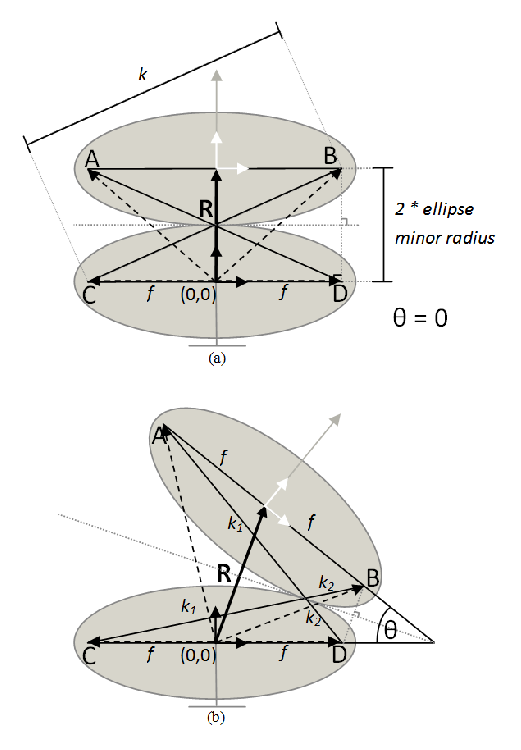
\includegraphics[width = 0.9\columnwidth]{figures/starry3.eps}
	\caption{Diagrams (a) and (b) show the trigonometric relationships employed in the adduction/abduction plane of motion of the Bi-Ellipsoidal CMC joint. Points A,B,C,D correspond to vectors $\mathbf{a,b,c,d}$, which are shown as dashed vectors that terminate at the foçi of the ellipses. Subsequent kinematic frames are shown in black and white at the centers of the ellipses. 
	}\label{spacesymbol}
	%%
\end{figure}

Once we have incorporated both major and minor radii definitions into the general form of an ellipse, the center to focus distance, $f$, is defined as shown in Figure \ref{spacesymbol}. The 2D joint is first shown in part (a) of Figure \ref{spacesymbol} at its neutral position of abduction/adduction, which corresponds to $\theta = 0$. The coordinate equation defining an ellipse is shown in Equation \ref{garden} \cite{wolf}. The constant length $k$ is defined in Equation \ref{eqk}. Equation \ref{pythagarino} is produced as a result of the Pythagorean Theorem about the right-triangle BDC. Re-arranging Equation \ref{pythagarino} in Equation \ref{ff}, the constant length $f$ is defined in Equation \ref{eqf}. Part (b) of Figure \ref{spacesymbol} extends this formulation by showing the joint during motion at any non-zero angle, where the axis of joint motion is defined by $\theta$. 

\begin{equation} 
%\hspace{40pt} 
4 f^{2} = 4 r_{major}^{2} - 4 r_{minor}^{2} 
%\hspace{40pt} 
\label{ff}
\end{equation}

\begin{equation} 
%\hspace{40pt} 
f = \sqrt{r_{major}^{2}-r_{minor}^{2}}
%\hspace{40pt} 
\label{eqf}
\end{equation}

In Equations \ref{eq10}-\ref{eq13}, four internal angles are defined using the points shown in Figure \ref{spacesymbol}; as these angles are all coupled to the motion of the joint, $\theta{}$:

\begin{equation} 
%\hspace{40pt} 
\angle BDC = \frac{\pi + \theta}{2}
%\hspace{40pt} 
\label{eq10}
\end{equation}

\begin{equation} 
%\hspace{40pt} 
\angle ADB = \arcsin (\frac{2 f \sin \angle BDC}{k})
%\hspace{40pt} 
\label{eq11}
\end{equation}

\begin{equation} 
%\hspace{40pt} 
\angle ADC = \angle BDC - \angle ADB
%\hspace{40pt} 
\label{eq12}
\end{equation}

\begin{equation} 
%\hspace{40pt} 
\angle BCD = \pi - \angle BDC - \angle ADB
%\hspace{40pt} 
\label{eq13}
\end{equation}

Once all necessary angles have been defined, the parametric equations to describe the vectors that locate the foçi of both ellipses, $\mathbf{a,b,c,d}$, appear in Equations \ref{eq14}-\ref{eqD}.

\begin{equation} 
%\hspace{40pt} 
\mathbf{a} = \begin{bmatrix} f - k \cos \angle ADC \\ k \sin \angle ADC \end{bmatrix}
%\hspace{40pt} 
\label{eq14}
\end{equation}

\begin{equation} 
%\hspace{40pt} 
\mathbf{b} = \begin{bmatrix} -f + k \cos \angle BCD \\ k \sin \angle BCD \end{bmatrix}
% \mathbf{b} = (-f + k \cos \angle BCD, k \sin \angle BCD) %MAKE ONE COLUMN
%\hspace{40pt} 
\label{eq15}
\end{equation}

\begin{equation} 
%\hspace{40pt} 
\mathbf{c} = \begin{bmatrix} -f \\ 0 \end{bmatrix}
%\hspace{40pt} 
\label{eqC}
\end{equation}

\begin{equation} 
%\hspace{40pt} 
\mathbf{d} = \begin{bmatrix} f \\ 0 \end{bmatrix}
% \mathbf{b} = (-f + k \cos \angle BCD, k \sin \angle BCD) %MAKE ONE COLUMN
%\hspace{40pt} 
\label{eqD}
\end{equation}

Vectors $\mathbf{a}$ and $\mathbf{b}$ are the position vectors of the points $\mathbf{A}$ and $\mathbf{B}$, as shown in Figure \ref{spacesymbol}, in the frame shown in black whose origin is at the center of the stationary ellipse. While it could be useful in certain cases to continue the kinematic chain and simply define vector $\mathbf{a}$ or $\mathbf{b}$ as the next linkage of the robot, we define the origin of the next forward kinematic frame as occurring at the center of the mobile ellipse, as shown in white in Figure \ref{spacesymbol}. 

\begin{equation} 
%\hspace{40pt} 
\mathbf{R} = \Biggr[ \begin{matrix} \overline{ \mathbf{a_x,b_x}} \\ \overline{ \mathbf{a_y,b_y}} \end{matrix} \Biggr]
% \mathbf{b} = (-f + k \cos \angle BCD, k \sin \angle BCD) %MAKE ONE COLUMN
%\hspace{40pt} 
\label{rrr}
\end{equation}

Vector $\mathbf{R}$ is the vector between ellipses' centers, as well as in the 3D model between the ellipsoids centroids; in both cases, it functions as an intermediate frame which splits the angular motion at the CMC joint between itself and the previous frame, which is located at (0,0) in Figure \ref{spacesymbol}. This vector is shown both in black in Figure \ref{spacesymbol} and in green in Figure \ref{2dc}. Vector $\mathbf{R}$ is defined as the mean of vectors $\mathbf{a}$ and $\mathbf{b}$ as shown in Equation \ref{rrr}, and it also defines the motion of the center point of the upper ellipse. The kinematic modeling of the gimbal joint is outlined in Table \ref{tabl}. Both the gimbal and the Bi-Ellipsoidal models' abduction/adduction tendons terminate past the CMC joint. Their flexion/extension tendons continue further and thus are coupled with motion at both the CMC joint and the IP joint, terminating near the fingertip on the Distal Phalanx (DP). 


\subsection{Comparison via Denavit-Hartenberg Parameters}
\label{dhsection}

It should be noted that for both the planar and spatial cases of identical spheres (but not for identical ellipsoids), a rolling without sliding relationship has been effectively demonstrated in a prototype robotic wrist and elbow joint \cite{Koreatech-arm}, \cite{lims2}. Drawing from this idea, our design and prototypes represent the first design considered that allows the generalization of the joint surface geometries from spheres to ellipsoids. This primarily allows our model to tune the major and minor radii to select the best available geometry of ellipse for any given joint. %This also means our model can create varied workspace geometries and Manipulability Metrics by varying the radii of the ellipsoids which are orthogonal to the finger at the CMC joint: as ellipsoids' radii vary in 3D-space and spheres' are the same in all directions, by varying the oblate or prolate aspect of the ellipsoids. %, it is possible to embody this kinematic model in anthropomorphic models of other complex joints that provide two degrees of freedom to the controller of the device. %If rigid beams are used to link the foçi, this mechanism is equivalent to linking two meshed gears together, where the ellipses' surfaces represent the interface of both gears. 

By bringing the rolling-ellipse relationship in 2D into any possible pose's cross-section in 3D, an ellipsoidal relationship can similarly be built which incorporates rolling over the surface. This solves the challenge of co-located joints: by having two ellipsoids roll over one another, the location is shared without compromising the resistance to compressive reaction forces. For example, reaction forces which would impart a shear load on the gimbal joint's pins would be better managed by the Bi-Ellipsoidal joint, which distributes the contact force into the palm. The Denavit-Hartenberg parameters of the thumb with the ellipsoidal rolling CMC joint and a gimbal CMC joint are outlined in Table \ref{tabl}. A virtual prismatic joint is used to represent the translation of the center of the moving ellipse as it rolls without slipping. Interestingly, these DH parameters can represent both the gimbal CMC joint, and the Bi-Ellipsoidal CMC joint: the gimbal CMC joint is just a special case of the Bi-Ellipsoidal case, as the gimbal CMC joint is the case where $\mathbf{R}$ goes to zero. Looking at the kinematics outlined by the Denavit-Hartenberg parameters in Table \ref{tabl}, the Bi-Ellipsoidal parameters are identical to the gimbal parameters, for the case that $\mathbf{R = 0}$: the kinematic models still work for this condition, and the although they require some extra frames to calculate as compared to the more direct kinematic model for a gimbal joint. Table \ref{tabl} shows variables $\mathbf{\mu}$ and $\mathbf{\sigma}$ respectively representing the motions of Flexion/Extension and Abduction/Adduction, which co-locate at the CMC joint. Because of the MCP joint's arthrodesis, no motion occurs. Finally, the IP joint is modeled as having a normal range of motion in the Distal Phalanx, as represented by variable $\mathbf{\omega}$ in Table \ref{tabl}.


%REORDER COLUMNS by CRAIG ... DONE!
\begin{table}
	\centering
	\caption{Denavit-Hartenburg (DH) Parameters for transformation matrices $M_i$. Angle measurements are shown in degrees.}
		\begin{tabular}{c|c|c|c}
		$\alpha_{i-1}$ & $a_{i-1}$ & $d_i$ & $\theta_i$ \\
		\hline
		(deg.) & (mm) & (mm) & (deg.) \\
		Rot. $x_{i-1}$ axis & Tran. $x_{i-1}$ axis & Tran. $z_i$ axis & Rot. $z_i$ axis \\
		\hline
		\hline
 -90$\degree$ & 0 & 0 & $\mu$/2$\degree$\\
 90$\degree$ & 0 & 0 & 90$\degree$+$\sigma$/2$\degree$\\
 -90$\degree$ & 0 & R & 0$\degree$\\
 90$\degree$ & 0 & 0 & -90$\degree$+$\sigma$/2$\degree$\\
 -90$\degree$ & $\ell_{mcp}$ & 0 & $\mu$/2$\degree$\\
 90$\degree$ & 0 & 0 & 10$\degree$\\
 -90$\degree$ & $\ell_{pp}$ & 0 & 15$\degree$\\
 0$\degree$ & 0 & 0 & $\omega\degree$\\
 0$\degree$ & $\ell_{dp}$ & 0 & 0$\degree$\\
 \hline
 \hline
	\end{tabular}
	\label{tabl}
\end{table}

\section{Data Collection Procedure}
\label{datasection}

%To ensure catch-points (where the tendon path is erroneously interrupted) and other displacements are measured when the prototype's motion is being recorded, the flexion, extension, adduction, and abduction tendons were all measured synchronously to produce an accurate numerical representation of the Jacobian (and thus the Manipulability Metric) at each point.
The tip of the thumb was moved throughout its workspace, involving both the IP joint and the 2-DOF CMC joint, and the excursions of the four tendons were recorded. Data was collected at 240 Hz using a {\it Saleae Logic} signal recorder. The base of the thumb was mounted to the lab bench, with the tendons connected to carriages on linear slides (shown in Figure \ref{experiment}) similar to those used in the experiments of Rake \cite{rake2}. The tendons are attached to weighted springs that pass through Teflon tubes that run through the PLA lab stand, shown in gray in Figure \ref{thumbcatch}, before re-entering the MCP Fusion. One carriage is attached to each tendon and moves with it; with the gravitational load on the weights, the carriages follow the movements of the thumb without the tendons ever going slack. The position of the carriages was measured using Avago encoders with US Digital encoder strips supplying 158 edges per centimeter. Use of a magnetic orientation sensor, {\it Polhemus Liberty}, was employed to track the $x$, $y$, and $z$ coordinates and orientation of the thumb tip in the base frame through its workspace. The end effector data was in Cartesian space with Euler angles, and the system also reported for each data point a Polhemus sensor quality metric that consistently indicated measurements collected were free from significant distortion. All components that are relevant are shown in Figure \ref{experiment}. If the tendon path is erroneously interrupted due to collision with an unexpected surface somewhere along its length, it is recorded as a ``catch point" in the data.

When finding all possible Manipulability Metrics across all possible poses of the thumb, each pose has a corresponding forward kinematics solution in the task space, upon which the MM value has been superimposed graphically in Figures \ref{analyticplot} and \ref{experimentplot}. For all four plots, the relative magnitude of these values is represented by the color of each dot at each point-cloud.
%The prevalence of such materials in the environment where a robotic hand would be deployed means this test is restricted to the lab environment, which is more controllable, for now. 

\begin{figure}
	%%%{7pt}
	\centering
	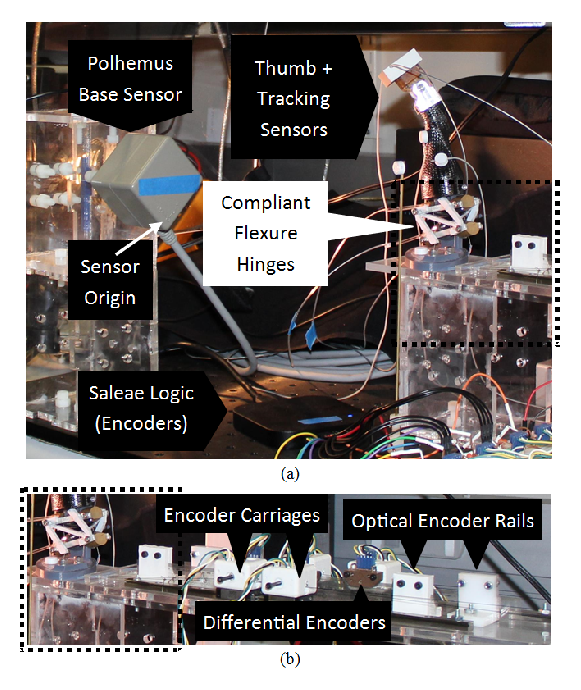
\includegraphics[width = 1\columnwidth]{figures/polhemus_and_setup.eps}
	\caption{(a) shows the workspace of the robotic thumb, the magnetic wired Polhemus sensors and base sensor, and Saleae logic analyser used to capture the displacement of the tendons. The origin of the base's magnetic field is printed on top of the base (gray box). The sensors remained proximal to the elevated base, such that surrounding objects did not interfere with the sensing. (b) shows the connected array of four white PLA carriages on clear linear rails, each with a differential optical encoder to track the displacement of the carriage over time.}
 \label{experiment}
	%%
\end{figure}

\begin{figure}
	\centering
	\includegraphics[width = 0.8\columnwidth]{figures/open-grasp.eps}\\
	%%
	\caption{(a) The Bi-Ellipsoidal CMC joint and Arthrodesized MCP joint mounted on the TU Hand, shown with the thumb in its neutral position. (b) The same prototype being used to grasp a stapler vertically.}\label{handgrasp}
	%%

\end{figure}

\begin{figure}
	\centering
 %%{7pt}
	\includegraphics[width = 1\columnwidth]{figures/analyticalmodels.eps}
	\caption{Joint Space to Task Space Manipulability Metric Comparison: The color shows the value of the Manipulability Metric as calculated for all regions of the thumb-tip's workspace.}\label{analyticplot}
	%%
\end{figure}

\begin{figure}
	\centering
 %%{7pt}
	\includegraphics[width = 1\columnwidth]{figures/experimentaldata.eps}
	\caption{Tendon Excursion To Task Space Manipulability Metric Comparison: The color shows the value of the Manipulability Metric as calculated for all regions of the thumb-tip's workspace.}\label{experimentplot}
	%%
\end{figure}


\section{Results}
\label{results}

The Manipulability Metrics were calculated for four cases, as shown in Figures \ref{analyticplot} and \ref{experimentplot}, with the following results: 

%\hspace{58pt}
\begin{itemize}
 \item Tendon manipulability (ellipsoidal):   \hfill         $\mathbf{1.0e{\text -}3}$
 \item Tendon manipulability (gimbal):        \hfill
 $\mathbf{3.1e1}$
 \item Standard manipulability (ellipsoidal): \hfill         $\mathbf{2.3e{\text -}3}$
 \item Standard manipulability (gimbal):      \hfill         $\mathbf{2.5e{\text -}3}$
\end{itemize}


\subsection{Joint Space to Task Space Manipulability Metric}

For the analytical cases, as seen in Figure \ref{analyticplot}, the manipulability metric was calculated numerically using finite differences on a grid of points in the workspace, achieved by evaluating the forward kinematics at a grid of points in the joint space. A crescent-shaped sub-region of the workspace can be visually identified as having a higher Manipulability Metric than elsewhere in the workspace. Comparing the output graphics of the gimbal CMC joint and the Bi-Ellipsoidal CMC joint, we see that the volume and size of the high-MM regions are similar, but the shape differs between the two: the region is noticeably wider and more bulbous at the ends of the Bi-Ellipsoidal CMC joint. In addition, the entire Bi-Ellipsoidal workspace appears somewhat wider and thinner.

One can also observe from the resulting workspace visualizations of the Manipulability Metric workspace shape that the models are kinematically similar, and while there is no major effect on the magnitude of MM at any given point, the Bi-Ellipsoidal model does result in a more distributed region of high-MM values. As shown in insets (b) and (c) of Figure \ref{analyticplot}, the highest density of high-MM values appear to be near the far side of the workspace, just above the metacarpal phalanges of the fourth and fifth fingers. These insets also show that the high-MM values appear to be in an elongated region in the Bi-Ellipsoidal case as compared to the traditional (gimbal) hinge-joint case in Figure \ref{2dc}. To the authors' knowledge, there has not yet been a comparable human study of thumb manipulability across the entire workspace. However, anyone may consider this possibility based on the simple observations of one's own thumbs, by observing what thumb positions permit the greatest degree of thumb tip rotations, while requiring as little translation as possible. 


\subsection{Tendon Extension to Task Space Manipulability Metric}

To calculate the tendon-to-task space Jacobian $J_T$, a cubic grid of approximately $30,000$ points $p_i \in W$ were chosen from within the workspace to help localize and aggregate the values of the $120,000$ data points collected. The Jacobian was computed from the experimental data at each of these cubic grid points. A linear regression was performed on the experimental data points (each of which had position data in the task space and associated tendon excursions) within a neighborhood $\mathcal{N}$ of each $p_i$. $\mathcal{N}$ consists of all points $p_j$ whose Euclidean distance from $p_i$ is less than a specific threshold: if the points are close enough to one another, the joint angles can only change by a small amount, and $J_T$ is nearly constant over all $p_j$ in $\mathcal{N}$.

From this Jacobian, the Manipulability Metric at each point was calculated across the workspace, from the standpoint of the tendon excursions, rather than from joint angles, and its magnitude is represented by color intensity. The color intensity is uniform over the region, with the exception of the edges of the workspace. As the mechanical stop simply truncates the non-joint-limited workspace at an arbitrary boundary, there is no mathematical reason to see high values there. For this reason, any high values are likely due to catch points or bouncing on the encoders as the thumb encounters the mechanical stop. This suggests that from the standpoint of tendon excursions, the Manipulability Metric is more uniform when calculated for tendon displacement than for joint angle displacement.


\section{Discussion}
\label{discussion}

The experimental plots shown in Figure \ref{experimentplot} and the analytical plots shown in Figure \ref{analyticplot} show the results of calculating the Manipulability Metric for a field of points in the thumb's workspace, and both figures use the same data processing technique. These four workspace color mappings appear to indicate that the Tendon Excursion To Task Space Manipulability Metric is somewhat consistent over the workspace, at least within the joint limits considered for a bioinspired thumb. These joint limits are similar to those in humans, so for a human-like range of motion the manipulability values are low and consistent: this further indicates that no large motions should suddenly result from small tendon excursions in certain locations of the workspace.

The fixated joint at the thumb model's MCP joint restricts the size of the dense central region of high MM values, which is best seen in the two analytical models shown in Figure \ref{analyticplot}. If MCP joint motion was allowed, a larger central region of high MM values would likely be observed. However, this doesn't say for certain that a larger size of the region of high manipulability would inherently be more practically useful, nor justify the additional cost and complexity. The Manipulability Metric data is recorded as a comparison between the proposed Bi-Ellipsoidal and the traditional design, so that the relative merits of underactuated designs can be robustly compared; this is possible because manipulability can be directly expanded into a family of formal indices known as the Manipulability Indices \cite{patel}, \cite{sptxt}. One example of applied manipulability indices is to predict how the kinematics of any thumb-like manipulator influence its ability to navigate a smartphone \cite{Endo}. However, within all current variations of these indices, there is a tacit assumption that each and every joint in the manipulator is actuated, where as this paper considers the manipulability when an arthrodesis at the MCP joint is applied. 

Despite being underactuated, our system still is analytically predicted to have a central region of the Joint Space to Task Space Manipulability Metric values that are around one order of magnitude higher than other regions in the workspace, for both the gimbal CMC joint and Bi-Ellipsoidal CMC joint prototype cases: this is because the CMC joint's range of motion is increased, compared to human range of motion, to counter-act the loss of workspace volume from fixating the MCP joint. Compare this to other regions in the workspace, where large changes in joint angles may result in only slight changes in the task space. It should be noted that the joint-angle Jacobian does not capture any information about the changes in length of the tendons as the thumb moves due to changing tendon pathway lengths, and so does not represent the inputs and outputs of the system as it is operated in practice: for this, the Tendon Excursion To Task Space Manipulability Metric represents a better measure. In either case, a relatively consistent manipulability over the workspace is a benefit, because it reduces the need to move some of the tendons over a large displacement in some regions while moving very small distances in others, which can be difficult to precisely actuate in operation of the hand during grasping. % If tendons cannot be precisely controlled at those poses, it may not be practical to manipulate objects with a tendon-driven device; however, we have observed that very few manipulation tasks occur with the thumb nearly right up against the palm.

This central region of high MM values is most apparent in the analytical plots of Figure \ref{analyticplot}, and can be seen up close to highlight its geometry: its apparent crescent shape is due to elevated Manipulability Metric values in that region. However, this region does not appear in the plots generated by tendon displacement, suggesting that the relationship between the joint space and the tendons are possibly inverting any region of elevated manipulability. At poses within the high-manipulability region, small changes in joint angles or tendon displacements can thus cause relatively small motions in task space; however, near poses outside this region, small changes in joint angles or tendon displacement may cause larger, undesired motion in task space. 

\begin{figure}
	\centering
	\includegraphics[width = 0.9\columnwidth]{figures/gimbal_model_catch.eps}\\
	
	\caption{The zoomed region (inset) shows a likely catch point occurring at the exposed flexion tendon as it crosses the CMC joint region during a movement test. On the gimbal CMC joint thumb prototype, the difference between the ideal-theoretical gimbal and that which can be assembled in a realistic manner is shown: while the gimbal CMC joint's kinematics do not require any volume to be accounted for by the device itself, a physical 2-DoF system must be embodied in a system of volumetric bodies. }
 \label{thumbcatch}
	%%
\end{figure}

While a gimbal is considered kinematically to consist of two rotational axes meeting at a point, in applications the components of which it is compromised take up physical space, which affects how practical they are in these applications: in practice their range of motion is limited and tendons cannot pass through the gimbal hardware, as shown in Figure \ref{thumbcatch}. To make the gimbal small, small shafts need to be used, which are in danger of shearing when loads are applied to the thumb. The ellipsoids offer a kinematically more stable tendon-driven thumb: the tendon paths vary with pose, which makes catch points and tendon collisions difficult to predict. Should the tendons catch on the ellipsoids, the smooth rolling motion distributes the tendons away from potential catch points, while the gimbal does not.

In summary, when compared to the Bi-Ellipsoidal CMC joint variant, the manipulability of the gimbal CMC joint thumb prototype appears to be of a smaller characteristic high-manipulability region when visualized in the workspace: both in terms of the shape of the region and the elevated values which comprise the regions themselves, as seen in Figures \ref{analyticplot} and \ref{experimentplot}. These differences, while visually apparent, are more subtle in their effect. As presented in Section \ref{results}, the Manipulability Metric values differ, but are within an equivalent order of magnitude throughout the entire workspace for all cases considered, except for the tendon-derived gimbal case. This suggests that both thumb prototypes will perform similarly at grasping and manipulation tasks; however, the rolling ellipsoidal joint introduces several key benefits for a small kinematic sacrifice: these include a magnetic restoring force from the ceramic ellipsoids, a spring restoring force from the flexure hinges, resistance to compressive loads, and lower vulnerability to catch points.

Finally, the comparison of the tendon-based Manipulability Metric to the standard joint-angle based Manipulability Metric showed that both methods produce different results: while they are of similar magnitudes, the former showed relatively even manipulability, while the latter produced a key region of high manipulability. These results were comparable but not exact, as is predicted by their mathematical relationship: While most small local motions will map easily from joint angle space to tendon space, catch points still affect the tendon pathway's length in practice, causing performance to deviate from that predicted by any theoretical kinematic model. When operating the gimbal CMC joint prototype, the edges of the aluminum were observed to contact the moving tendons, leading to catch points and subsequent noise in the displacements of the tendons. If there is elasticity in the tendons, it was not significant enough to be measured as a contribution to any major discrepancies. 

\section{Conclusion}
\label{conclusion}

We constructed a rolling ellipsoidal CMC joint on an underactuated thumb with proportions similar to a human, with flexion-extension and abduction-adduction axes collocated. Due to the contact between the magnets, the compliant mechanism was capable of resisting high contact forces. The position and orientation of each link, along with the tendon excursions, were recorded as the thumb was moved throughout its workspace. Next, we calculated and compared the standard Manipulability Metric and a tendon excursion-based metric. Two underactuated anthropomorphic thumb designs were studied: the gimbal CMC joint model and the Bi-Ellipsoidal joint model. For each of these thumb designs, we analytically determined the forward kinematics from joint space to task space, and experimentally characterized the tendon-to-task space kinematics. Application of the Manipulability Metric to each model shows that the predicted region of highest manipulability within the thumb-tip's workspace is a well-defined region of the thumb's workspace. In both models, this region occurs just above the metacarpal phalanges of the fourth and fifth fingers, which is where the most common prehensile grasps require the highest manipulability. The shape of this region differs slightly between the two designs, with the Bi-Ellipsoidal forward kinematics producing a more oblong result, but with similar volume.

Either prototype is predicted to produce similar performance in terms of manipulability; however, the Bi-Ellipsoidal CMC joint has many practical advantages. First, it is able to better withstand the axial transmission of forces about the joint than an equivalent gimbal CMC joint, which would experience an equivalent loading as much higher shear forces on the cross-sections of its hinge joint pins. Second, a physical gimbal will always take up extra surrounding space to build, which limits the relative range of motion as compared to the Bi-Ellipsoidal CMC joint. Finally, the ellipsoidal joint has better tendon management: for an equivalent range of adduction/abduction and flexion/extension motion, there are fewer inherent catch points in the Bi-Ellipsoidal model, as the tendons can slide smoothly over the ellipsoidal surface when in contact.

Suggestions for future work include creating an analytical model for the forward kinematics of the tendon excursions, and checking computationally for catch points in the model. This would allow us to analyze the tendon/joint space Jacobian at various poses analytically, elucidating further the relationships seen between the two models: this could determine whether the actual tendon behavior matches our models' assumptions. To do this, specific couplings between each joint angle and its neighboring tendon excursions must be determined: this is an arc-length calculation for hinge joints, and a comparable calculation for the Bi-Ellipsoidal joint. 

\section*{Acknowledgments}
Thanks to Albert Okoh and Dipayan Das for their dedicated work on manufacturing small robotic parts for this research.

\begin{thebibliography}{1}
\bibliographystyle{IEEEtran} 


%NOTE: The use of the tag `%0000' below is quality control: this means it's been cited parenthetically at least once, so that no references are provided that are not called.

%[1] - 
\bibitem{moravec} H. Moravec, Mind children: The future of robot and human intelligence. Harvard University Press, 1988.
%0000

%[2]
\bibitem{Martell} M. Martell, J. C. Diaz, and J. Schultz. "A Linear Multiport Network Approach for Elastically Coupled Underactuated Grippers." ASME Journal of Mechanisms and Robotics, 2017.
%0000

%[3]
\bibitem{Fuzzy}Y. Zhang, X. Xu, R. Xia and H. Deng, "Stiffness-Estimation-Based Grasping Force Fuzzy Control for Underactuated Prosthetic Hands," in IEEE/ASME Transactions on Mechatronics, vol. 28, no. 1, pp. 140-151, February 2023.
%0000

%[4]
\bibitem{Pulleyking} S. Pulleyking, D. Das and J. Schultz, "Simplified robotic thumb inspired by surgical intervention," 6th IEEE International Conference on Biomedical Robotics and Biomechatronics (BioRob), Singapore, pp. 1200-1206, 2016.
%0000

%[5]
\bibitem{Pulleyking-Schultz} S. Pulleyking and J. Schultz, "Flexure Hinge-based Biomimetic Thumb with a Rolling-Surface Metacarpal Joint," IEEE International Conference on Robotics and Automation (ICRA), Paris, France, pp. 2960-2966, 2020.
%0000

%[6]
\bibitem{Das-TUHand} D. Das, N. Rake, and J. Schultz. "The TU Hand: Using Compliant Connections to Modulate Grasping Behavior" In Robotic Grasping and Manipulation, RGMC 2016. Communications in Computer and Information Science, vol 816, 2018.
%0000

%[7] 
\bibitem{anatomy-textbook} A. M. R. Agur and A. Dalley. Grant's atlas of anatomy. Lippincott Williams and Wilkins, 2009.
%0000

%[8] 
\bibitem{noparams} A. M. Hollister, W. L. Buford, L. M. Myers, D.J. Giurintano, and A. Novick, "The axes of rotation of the thumb carpometacarpal joint." Journal of Orthopaedic Research, vol. 10, no. 3, pp. 454-460 1992.
%0000

%[9] 
\bibitem{reuleaux} A. Synek, M. Settles, and G. Stillfried, "Multi-body simulation of a human thumb joint by sliding surfaces." Proceedings of the IEEE Robotics Automation Letters and EMBS International Conference on Biomedical Robotics and Biomechatronics, pp. 379-384 2012.
%0000

%[10]
\bibitem{ShadowHand} D. Sharma, K. Tokas, A. Puri, and Krishna Sharda. "SHADOW HAND." Journal of Advance Research in Applied Science, vol. 1, no. 1, 2014.
%0000

%[11]
\bibitem{iCub} A. Schmitz, U. Pattacini, F. Nori, L. Natale, G. Metta and G. Sandini, "Design, realization and sensorization of the dexterous iCub hand," 10th IEEE-RAS International Conference on Humanoid Robots, pp. 186-191, 2010.
%0000

%[12]
\bibitem{KITECH-Hand} D. H. Lee, J. H. Park, S. W. Park, M. H. Baeg and J. H. Bae, "KITECH-Hand: A Highly Dexterous and Modularized Robotic Hand," in IEEE/ASME Transactions on Mechatronics, vol. 22, no. 2, pp. 876-887, April 2017.
%0000

%[13]
\bibitem{DLRhand} H. Liu et al., "Multisensory five-finger dexterous hand: The DLR/HIT Hand II," IEEE/RSJ International Conference on Intelligent Robots and Systems, Nice, France, pp. 3692-3697, 2008.
%0000

%[14]
\bibitem{schunkhand} F. Ficuciello, A. Federico, V. Lippiello, and B. Siciliano. "Synergies evaluation of the SCHUNK S5FH for grasping control." Advances in Robot Kinematics 2016, pp. 225-233. Springer, Cham, 2018.
%0000

%[15]
\bibitem{bebionic} J. T. Belter, and A. M. Dollar. "Performance characteristics of anthropomorphic prosthetic hands." 2011 IEEE International Conference on Rehabilitation Robotics, pp. 1-7. IEEE, 2011.
%0000

%[16]
\bibitem{AdaptUnderact} T. Yang, N. Sun, H. Chen and Y. Fang, "Adaptive Optimal Motion Control of Uncertain Underactuated Mechatronic Systems With Actuator Constraints," in IEEE/ASME Transactions on Mechatronics, vol. 28, no. 1, pp. 210-222, February 2023.
%0000

%[17]
\bibitem{softrigid} W. Zhu et al., "A Soft-Rigid Hybrid Gripper With Lateral Compliance and Dexterous In-Hand Manipulation," in IEEE/ASME Transactions on Mechatronics, vol. 28, no. 1, pp. 104-115, February 2023.
%0000

%[18]
\bibitem{Yoshikawa} T. Yoshikawa, "Manipulability of Robotic Mechanisms", The International Journal of Robotics Research, 1985.
%0000

%[19]
\bibitem{yokokohjiDME} Y. Yokokohji, J. S. Martin and M. Fujiwara, "Dynamic Manipulability of Multifingered Grasping," in IEEE Transactions on Robotics, vol. 25, no. 4, pp. 947-954, Aug. 2009.
%0000

%[20]
\bibitem{fhdef} Xu N, Dai M, Zhou X. Analysis and design of symmetric notch flexure hinges. Advances in Mechanical Engineering. vol 9, no. 11, 2017.
%0000

%[21] 
\bibitem{Blake} E. M. Blake, “Upon the Ruled Surfaces Generated by the Plane Movements Whose Centrodes Are Congruent Conics Tangent at Homologous Points.” American Journal of Mathematics 21, no. 3: pp 257–69. 1899. 
%0000

%[22]
\bibitem{MLS} R. M. Murray, Z. Li, and S. Sastry. A mathematical introduction to robotic manipulation. CRC press, 2017.
%0000

%[23]
\bibitem{malhotra} M. Malhotra and Y. Matsuoka, "The relationship between actuator reduction and controllability for a Robotic Hand," 2010 3rd IEEE RAS and EMBS International Conference on Biomedical Robotics and Biomechatronics, pp. 331-336, 2010.
%0000

%[24]
\bibitem{Rake-Tendons} N. J. Rake, S. P. Skinner, G. D. O'Mahony and J. A. Schultz, "Modeling and implementation of a simplified human tendon structure in a robotic finger," 6th IEEE International Conference on Biomedical Robotics and Biomechatronics (BioRob), pp. 120-125, 2016.
%0000

%[25]
\bibitem{rake2}  N. J. Rake, "A four-tendon robotic finger with tendon transmission inspired by the human extensor mechanism." Bioinspiration and Biomimetics, vol. 16, no. 4, 2021.
%0000

%[26]
\bibitem{thingiverse} Cohl. "Elliptical Gear with no center pivot". Thingiverse, 3D print file. Gears: Ellipsoidal Cross-foçi Linkage Demonstration, 2015.
%This rolling-ellipse relationship has been realized in hardware for kinematic demonstrations but not for any robotic devices \cite{thingiverse}. The rolling-ellipse relationship is the 2D case; the 3D case is the rolling-ellipsoid relationship; it has not yet been realized in hardware for either purpose.

%[27] 
\bibitem{springer2020} G. Glaeser, "Kinematics: Geometry in motion." In Geometry and its Applications in Arts, Nature and Technology, Springer, pp. 415-458. 2020.
%0000

%[28]
\bibitem{wolf} E. W. Weisstein, “Ellipse.” Wolfram MathWorld--A Wolfram Web Resource, 2023.
%0000

%[29]
\bibitem{Koreatech-arm}  Y. J. Kim, "Design of low inertia manipulator with high stiffness and strength using tension amplifying mechanisms." IEEE/RSJ International Conference on Intelligent Robots and Systems (IROS), pp. 5850-5856, 2015.
%0000

%[30] 
\bibitem{lims2} Y. J. Kim, J. I. Kim, and W. Jang. "Quaternion joint: Dexterous 3-DOF joint representing quaternion motion for high-speed safe interaction." IEEE/RSJ International Conference on Intelligent Robots and Systems (IROS), pp. 935-942, 2018.
%0000

%[31]
\bibitem{patel} S. Patel and T. Sobh. "Manipulator performance measures-a comprehensive literature survey." Journal of Intelligent and Robotic Systems, vol. 77, pp 547-570, 2015.
%0000

%[32]
\bibitem{sptxt} D. Prattichizzo, M. Pozzi, and M. Malvezzi. "Dexterous Manipulation." Encyclopedia of Robotics. Springer, Berlin, Heidelberg. 2020.
%0000

%[33] 
\bibitem{Endo} H. Endo, "Examination of robotic manipulability indices to evaluate upper limb manipulability in digital human models." International Journal of Human Factors Modelling and Simulation 6, no. 4, pp 282-297, 2018.
%0000

\end{thebibliography}

\newpage 

\section{Biography Section}

\vspace{11pt}

\begin{IEEEbiography}[{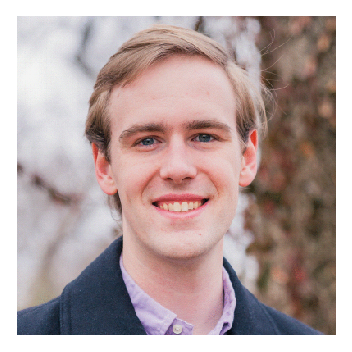
\includegraphics[width=1in,height=1.25in,clip,keepaspectratio]{figures/HeadshotSP.eps}}]{Spenser Pulleyking}
Is a Ph.D. Student at The University of Tulsa in the Department of Mechanical Engineering. He received a BSME degree from The University of Tulsa in Tulsa, OK. His research interest center on low-cost applications for robotic grasping, dexterous manipulation, and biomimetic soft/rigid hybrid robots.  
\end{IEEEbiography}

\vspace{11pt}

\begin{IEEEbiography}[{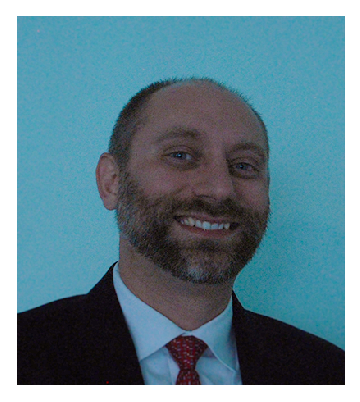
\includegraphics[width=1in,height=1.25in,clip,keepaspectratio]{figures/Headshot2020_450.eps}}]{Joshua Schultz}
Is Associate Professor at The University of Tulsa in the Department of Mechanical Engineering. He received the BSME degree from Tufts University in Medford, MA, the MS from Vanderbilt University, Nashville, TN, and the Ph.D. from Georgia Institute of Technology, Atlanta, GA. He was named an ARCS Scholar in 2011. His research interests center on biologically inspired paradigms for robotic motion, including artificial muscles, soft robotics, manipulation and grasping.
\end{IEEEbiography}

\vfill

\newpage

%\section*{Captions and}
%%
\listoffigures

\end{document}


